\documentclass[conference]{IEEEtran}
\usepackage{cite}
\usepackage{amsmath,amssymb}
\usepackage{graphicx}
\usepackage{booktabs}
\usepackage{multirow}
\usepackage{array}
\usepackage{url}
\usepackage{xcolor}
\usepackage{tikz}
\usetikzlibrary{arrows.meta,positioning}

% Figures and data tables are generated from the experiment results by make_figures.py
\graphicspath{{figures/}}
% the primitive \input is expandable, so generated table rows can be read inside a tabular
\makeatletter
\newcommand{\tabinput}[1]{\@@input #1 }
\makeatother

\begin{document}

\title{Does In-Domain Masked Autoencoding Overtake ImageNet Initialisation Under Label Scarcity?\\
Two Pre-Registered Studies Across Four Visual Domains}

\author{\IEEEauthorblockN{Namrata Pathak}
\IEEEauthorblockA{M.Tech in Artificial Intelligence and Data Science\\
KIIT University, Bhubaneswar, India\\
namratapathak0410@gmail.com}}

\maketitle

\begin{abstract}
For label-poor domains it is often suggested to skip ImageNet and pretrain on the domain's own unlabelled images.
We tested this for masked autoencoders (MAE) and a small Vision Transformer (ViT): as labels grow, when does a ViT
pretrained with in-domain MAE beat the same ViT started from ImageNet-1k weights, and does distance from ImageNet
tell us in advance? Two pre-registered studies covered four domains (plant disease, satellite, objects, animals),
leakage-safe splits, label budgets from 5 to 100\,\% and three seeds on one laptop GPU. In Study~1 (240 runs) the
ImageNet ViT won all 20 dataset--budget cells. The gap closed steadily with more labels but never reversed (on
PlantVillage from $-0.239$ to $-0.020$ macro-F1), and none of four domain distances predicted it (exact
$p \geq 0.33$). Study~2 (405 runs) removed three possible handicaps. A four times larger unlabelled pool did not
improve MAE (all differences within $\pm 0.02$), a wider learning-rate grid left ImageNet ahead in all 20 cells,
and ResNet-34 behaved like ResNet-18. Continuing MAE from the ImageNet weights was never significantly better than
ImageNet alone and was significantly worse in 10 of 20 cells. At this scale, ImageNet initialisation is the safer
default.
\end{abstract}

\begin{IEEEkeywords}
self-supervised learning, masked autoencoders, vision transformers, transfer learning, label efficiency,
domain distance, calibration, plant disease
\end{IEEEkeywords}

% =====================================================================================================
\section{Introduction}
Labels are the expensive part of most vision projects outside everyday photography. Anyone can photograph a
tomato leaf, but deciding which of a dozen diseases it shows takes a plant pathologist. Satellite land-cover maps
and medical scans have the same problem. So nobody trains from scratch; the usual first step is to load weights
learned on ImageNet~\cite{deng2009imagenet}, a collection of 1.28 million labelled photographs of everyday objects.

Self-supervised learning offers a second option. A masked autoencoder (MAE)~\cite{he2022mae} hides most of an
image's patches and trains the network to paint them back in. It needs no labels, so it can be run on exactly the
images one cares about. The choice is therefore between a lot of knowledge from the wrong visual world and a little
knowledge from the right one. Several papers report that MAE pretraining on small target datasets helps
ViTs~\cite{elnouby2021largescale,zhou2022selfpretrain,mao2022maedatahungry,das2024limited}, and in-domain
contrastive pretraining has been found to compete with ImageNet in some settings~\cite{cole2022contrastive}. What
we could not find is an answer to the practical question \emph{at what label budget} the in-domain route starts to
pay off, and whether one can tell in advance from how different the domain looks from ImageNet. Ericsson
et~al.~\cite{ericsson2021transfer} list exactly this link between domain distance and transfer as open.

We set out to answer it with a controlled, pre-registered design. Our contributions are:
\begin{enumerate}
\item A comparison of four starting points on four domains in which the three ViTs are architecturally identical
and differ only in their initial weights, trained on the same nested label subsets with the same protocol.
\item A crossover analysis over five label budgets. In-domain MAE never overtakes ImageNet, but the gap shrinks in
every domain as labels are added.
\item Four distances between each domain and ImageNet, measured before training. They disagree with one another
and none of them predicts the gap.
\item A follow-up study that removes three possible excuses for MAE (too little unlabelled data, a narrow
learning-rate grid, a weak convolutional baseline) and tests a hybrid that continues MAE from ImageNet weights.
None of these changes the conclusion.
\item Evidence that rankings by accuracy replicate across domains, whereas rankings by calibration after
temperature scaling do not.
\end{enumerate}
Both studies were written down and committed to a public repository before their first training run, and together
they took about 36\,h on a laptop GPU.

% =====================================================================================================
\section{Related Work}
\textbf{Transfer from ImageNet.} Models that do better on ImageNet usually transfer
better~\cite{kornblith2019transfer}, but Raghu et~al.~\cite{raghu2019transfusion} found that for medical images
much of what ImageNet pretraining provides is not needed. ViTs~\cite{dosovitskiy2021vit} lack the built-in locality
of convolutional networks~\cite{he2016resnet} and lean heavily on pretraining; DeiT~\cite{touvron2021deit} made it
possible to train them on ImageNet-1k alone.

\textbf{Self-supervised and in-domain pretraining.} Ericsson et~al.~\cite{ericsson2021transfer} showed that how well
self-supervised models transfer depends strongly on the target domain. Cole et~al.~\cite{cole2022contrastive} varied
the size and the domain of the pretraining set for contrastive ResNet-50 models. MAE~\cite{he2022mae} hides 75\,\%
of the patches and regresses their pixels. El-Nouby et~al.~\cite{elnouby2021largescale} and Zhou
et~al.~\cite{zhou2022selfpretrain} reported that masked pretraining on the target data alone can be competitive,
and Mao et~al.~\cite{mao2022maedatahungry} and Das et~al.~\cite{das2024limited} used MAE to make ViTs less data
hungry. Hammoud et~al.~\cite{hammoud2024diversity} looked at the role of diversity in the pretraining data.
Continuing to pretrain an existing model on in-domain data is a well-established idea in language
modelling~\cite{gururangan2020dontstop}, and Reed et~al.~\cite{reed2022hpt} found that self-supervised pretraining
started from ImageNet weights converges faster and transfers better than starting from scratch. On the plant side,
deep networks are highly accurate on PlantVillage~\cite{hughes2015plantvillage,mohanty2016plant}, and
self-supervised transformers have been trained on plant images~\cite{wang2024gpid}. We did not find a study that
locates the label budget at which in-domain MAE overtakes ImageNet across several domains.

\textbf{Dataset distance and calibration.} FID~\cite{heusel2017fid} compares two feature distributions, and
OTDD~\cite{alvarezmelis2020otdd} also accounts for the labels. Guo et~al.~\cite{guo2017calibration} showed that
modern networks are overconfident and proposed temperature scaling; Minderer et~al.~\cite{minderer2021calibration}
revisited the question for newer architectures, and Sambyal et~al.~\cite{sambyal2023calibration} studied
calibration with limited medical data. Dehghani et~al.~\cite{dehghani2021lottery} caution that conclusions drawn on
one benchmark often fail to carry over, which is why we use several domains and rank
statistics~\cite{demsar2006comparisons}.

% =====================================================================================================
\section{Method}

\begin{figure*}[t]
\centering
\resizebox{\textwidth}{!}{%
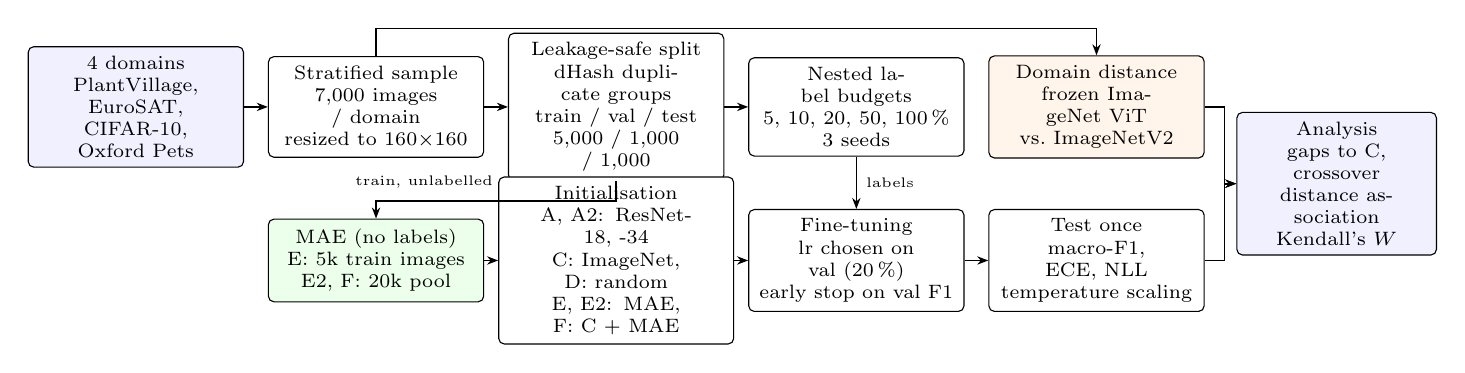
\begin{tikzpicture}[
  box/.style={draw, rounded corners=2pt, align=center, font=\scriptsize, text width=2.5cm, minimum height=1.05cm,
              fill=#1},
  box/.default=white,
  arr/.style={-{Stealth[length=4pt]}, semithick}]
\node[box=blue!6]   (data)   at (0,0)     {4 domains\\PlantVillage, EuroSAT,\\CIFAR-10, Oxford Pets};
\node[box]          (samp)   at (3.05,0)  {Stratified sample\\7,000 images / domain\\resized to 160$\times$160};
\node[box]          (split)  at (6.1,0)   {Leakage-safe split\\dHash duplicate groups\\train / val / test\\5,000 / 1,000 / 1,000};
\node[box]          (bud)    at (9.15,0)  {Nested label budgets\\5, 10, 20, 50, 100\,\%\\3 seeds};
\node[box=orange!8] (dist)   at (12.2,0)  {Domain distance\\frozen ImageNet ViT\\vs.\ ImageNetV2};
\node[box=green!8]  (mae)    at (3.05,-1.95) {MAE (no labels)\\E: 5k train images\\E2, F: 20k pool};
\node[box, text width=2.75cm] (init) at (6.1,-1.95) {Initialisation\\A, A2: ResNet-18, -34\\C: ImageNet, D: random\\E, E2: MAE, F: C + MAE};
\node[box]          (ft)     at (9.15,-1.95) {Fine-tuning\\lr chosen on val (20\,\%)\\early stop on val F1};
\node[box]          (test)   at (12.2,-1.95) {Test once\\macro-F1, ECE, NLL\\temperature scaling};
\node[box=blue!6, text width=2.3cm] (ana) at (15.25,-0.975) {Analysis\\gaps to C, crossover\\distance association\\Kendall's $W$};
\draw[arr] (data) -- (samp);
\draw[arr] (samp) -- (split);
\draw[arr] (split) -- (bud);
\draw[arr] (samp.north) -- ++(0,0.35) -| (dist.north);
\draw[arr] (split.south) -- ++(0,-0.25) -| node[pos=0.4, above=1pt, font=\tiny] {train, unlabelled} (mae.north);
\draw[arr] (mae) -- (init);
\draw[arr] (init) -- (ft);
\draw[arr] (bud) -- node[right, font=\tiny] {labels} (ft);
\draw[arr] (ft) -- (test);
\draw[arr] (test.east) -- ++(0.25,0) |- (ana.west);
\draw[arr] (dist.east) -- ++(0.25,0) |- (ana.west);
\end{tikzpicture}}
\caption{Pipeline, run separately for each domain. Study~1 uses arms A, C, D and E; Study~2 adds A2, E2 and F.
Only MAE pretraining sees images before fine-tuning, and never validation or test images. Each run is evaluated on
the test set once.}
\label{fig:pipeline}
\end{figure*}

\subsection{Arms}
Every arm is fine-tuned on the same labelled subsets (Fig.~\ref{fig:pipeline}). In Study~1 there are four.
\textbf{A} is a ResNet-18~\cite{he2016resnet} trained from random weights (11.2\,M parameters). \textbf{C} is a
ViT-Tiny with the DeiT-Tiny layout~\cite{touvron2021deit} (12 blocks, width 192, 3 heads, 5.5\,M parameters)
loaded with supervised ImageNet-1k weights. \textbf{D} is the same ViT from random weights, and \textbf{E} is the
same ViT whose weights come from an MAE trained on the domain's own training images, without their labels. Since
C, D and E have one architecture, any difference between them comes from the starting weights. Our main contrast is
E$-$C; E$-$D shows what MAE adds to a ViT, and E$-$A compares it with the inductive bias of a CNN.

Study~2 adds three arms. \textbf{E2} is E with a four times larger unlabelled pool. \textbf{F} starts from C's
ImageNet weights, continues MAE pretraining on the same pool, and is then fine-tuned like the others.
\textbf{A2} replaces ResNet-18 by ResNet-34 (21.3\,M parameters). We kept ViT-Tiny, small ResNets and 160\,px
inputs so that each study fits within 48\,h on one RTX~4050 Laptop GPU with 6\,GB of memory.

\subsection{Data, splits and label budgets}
Each domain is represented by one dataset (Table~\ref{tab:data}): PlantVillage~\cite{hughes2015plantvillage}
(plant disease, colour images), EuroSAT RGB~\cite{helber2019eurosat} (land cover from satellites),
CIFAR-10~\cite{krizhevsky2009cifar} (objects) and Oxford-IIIT Pets~\cite{parkhi2012pets} (cat and dog breeds). We
draw 7,000 images per dataset, stratified by class, so all domains start with the same amount of data. Images are
resized so that the shorter side is 160\,px (bicubic) and centre-cropped; CIFAR-10 and EuroSAT are upsampled in the
process.

Datasets such as PlantVillage contain many near-copies, for example several shots of the same leaf. If such copies
land on both sides of a split, test scores are inflated. We therefore hash every image (256-bit difference hash),
link images whose hashes differ in at most 10 bits, and keep each linked group inside one split. The 70/15/15 split
is made with \texttt{StratifiedGroupKFold} (seed 42). The label budgets are 5, 10, 20, 50 and 100\,\% of each
class's training images, with at least one image per class, which corresponds to roughly 250 to 5,000 labelled
images. Smaller subsets are contained in larger ones, and all arms see the same subset for a given seed. The seed
(0, 1 or 2) also fixes the order of the data, the initialisation of any new layers and the MAE run used by E.

\begin{table*}[t]
\centering
\caption{Datasets, leakage-safe splits and distances to ImageNet, measured before training. The arrow shows which
direction means ``farther from ImageNet''.}
\label{tab:data}
\footnotesize
\begin{tabular}{llccccrrrr}
\toprule
Dataset & Domain & Classes & Native px & Train/Val/Test & Dup.\ groups & FID $\uparrow$ & OTDD $\uparrow$ &
ImageNet conf.\ $\downarrow$ & Linear probe $\downarrow$ \\
\midrule
\tabinput{tables/datasets.tex}
\bottomrule
\end{tabular}
\end{table*}

\subsection{Distance between a domain and ImageNet}
We pass every image through the frozen ImageNet DeiT-Tiny of arm C and keep its 192-d class token. ImageNetV2
(matched frequency)~\cite{recht2019imagenetv2}, with 10,000 images over all 1,000 classes, stands in for ImageNet.
On the training split we compute four numbers. (i) FID~\cite{heusel2017fid} between the two sets of features.
(ii) OTDD~\cite{alvarezmelis2020otdd}, an optimal-transport distance in which the cost of matching two images also
depends on how similar their classes are; we use a diagonal Gaussian per class, 64 PCA dimensions and 1,500 samples
per side, solved with POT~\cite{flamary2021pot}. (iii) ImageNet confidence: the average top-class probability that
the 1,000-way ImageNet classifier assigns to the domain's images (0.458 on ImageNetV2 itself). (iv) The validation
accuracy of a logistic-regression probe trained on the frozen features. Large FID or OTDD, and small confidence or
probe accuracy, mean the domain is far from ImageNet.

\subsection{MAE pretraining}
The MAE encoder is exactly the ViT-Tiny used by the other ViT arms, so its weights drop straight into E. Of the
100 patches of an image, 75\,\% are hidden. A light decoder (2 blocks, width 128, 4 heads) predicts the
per-patch normalised pixels of the hidden patches. We use batch 256, AdamW with $\beta=(0.9,0.95)$, a base
learning rate of $1.5\times10^{-4}$, weight decay 0.05, a cosine schedule, random resized crops (scale 0.2--1) and
horizontal flips. Encoder position embeddings start from fixed 2-D sine--cosine values. For E the pool is the
$\sim$5,000 unlabelled training images, seen for 800 epochs (15,200 steps, 40 warm-up epochs). A separate MAE is
trained for each seed, which takes about 21.5\,min.

In Study~2 the pool grows to 20,000 images: the training images plus 15,000 extra images of the same dataset taken
from \emph{outside} the 7,000-image sample, so no validation or test image can enter it. As a further safeguard, we
drop any extra image whose hash lies within 10 bits of a validation or test image or of a flipped copy of one (227
images on EuroSAT, none elsewhere). E2 is trained for the same 15,200 steps as E with 760 warm-up steps, so only the
data changes, not the compute. F uses the same schedule but starts from the ImageNet weights, keeps their learned
position embeddings and uses a smaller learning rate of $5\times10^{-5}$ so as not to wipe out what ImageNet
taught. That value was fixed in advance and not tuned. Oxford Pets has no images beyond our sample, so there is no
E2 for Pets, and its F uses the 5,000 training images.

\subsection{Fine-tuning}
All arms follow Table~\ref{tab:setup}. The number of steps grows with the number $n$ of labelled images. We check
validation macro-F1 25 times per run, stop after 8 checks without improvement, restore the best checkpoint and only
then evaluate on the test set. Pretrained ViTs use layer-wise learning-rate decay of 0.75~\cite{bao2022beit}, so
that the early blocks move less than the late ones. The learning rate for each dataset and arm is picked on
validation macro-F1 at the 20\,\% budget with seed 0 and then reused for every budget and seed. Study~2 widens the
grid from three to five values (Table~\ref{tab:setup}) and retunes every arm. Where the choice for an old arm stays
the same, the Study~1 runs are reused; where it changes, those runs are repeated.

\begin{table}[t]
\centering
\caption{Fine-tuning protocol, shared by all arms unless stated otherwise.}
\label{tab:setup}
\footnotesize
\begin{tabular}{@{}ll@{}}
\toprule
Optimiser & AdamW~\cite{loshchilov2019adamw}, weight decay 0.05 \\
Batch / precision & 128 / bf16, gradient clipping 1.0 \\
Schedule & 5\,\% linear warm-up, cosine decay \\
Steps & $\mathrm{clip}(100\lceil n/128\rceil, 600, 4000)$ \\
Early stopping & 25 val.\ checks, patience 8, restore best \\
Augmentation & random resized crop 0.35--1, flip, \\
 & brightness/contrast $\pm$20\,\% \\
ViT details & drop-path 0.1, average-pooled tokens \\
Layer-wise lr decay & 0.75 (pretrained ViTs: C, E, E2, F) \\
LR grid, scratch & S1: $\{0.5, 1, 2\}\times10^{-3}$ \\
 & S2: $\{0.25, 0.5, 1, 2, 4\}\times10^{-3}$ \\
LR grid, pretrained & S1: $\{0.25, 0.5, 1\}\times10^{-3}$ \\
 & S2: $\{0.125, 0.25, 0.5, 1, 2\}\times10^{-3}$ \\
\bottomrule
\end{tabular}
\end{table}

\subsection{Metrics and statistics}
Test macro-F1 is the primary metric. For calibration we report the expected calibration error (ECE, 15 equal-width
bins~\cite{naeini2015ece,guo2017calibration}) before and after temperature scaling, with the temperature fitted on
validation data. Gaps between two arms are paired by seed, because both see the same labelled subset, and are given
with a 95\,\% $t$-interval over the three seeds. The crossover budget is where the mean gap changes sign, found by
interpolating on a log-budget axis. If the sign never changes we report the crossover as censored ($>$100\,\% or
$<$5\,\%), and we accept a crossover only if the intervals exclude zero on both sides of it. To summarise a dataset
with one number we average the gap over the log-budget axis (trapezoidal rule). We relate this mean gap to each
distance with Spearman's $\rho$, an exact permutation $p$-value and a leave-one-dataset-out linear prediction,
compared against simply predicting the mean of the other datasets. Four datasets allow no two-sided $p$ smaller
than $2/4! = 0.083$, so we declared this part exploratory from the start. Agreement of the arm rankings across
datasets is measured per budget with Kendall's $W$~\cite{kendall1939rankings} and the Friedman test.

\subsection{Pre-registration}
Study~1's hypotheses (H1--H5), protocol and analysis plan were committed to the repository before the first
training run. A single amendment, also made before training, raised MAE pretraining from 400 to 800 epochs once a
speed test showed that the budget allowed it. Study~2's hypotheses (H6--H11) were committed after Study~1 had
finished but before any Study~2 code was run. Table~\ref{tab:hyp} lists all eleven with their outcomes.

% =====================================================================================================
\section{Study 1: Results}
All 240 runs finished: 9.3\,h of fine-tuning, 1.0\,h of learning-rate selection and about 4.3\,h of MAE
pretraining, 14.6\,h in total, never using more than 3.4\,GB of GPU memory.

\begin{figure*}[t]
\centering
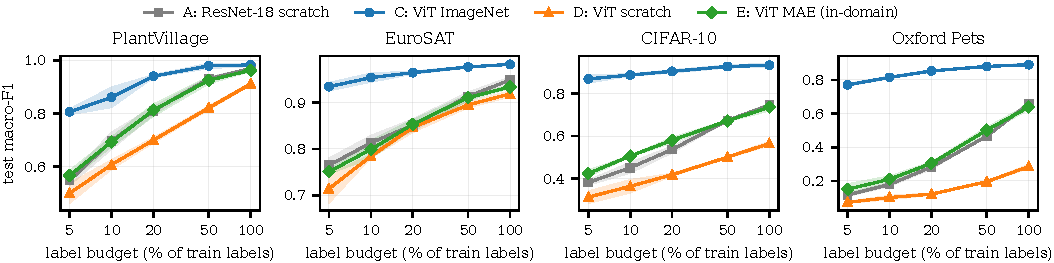
\includegraphics[width=\textwidth]{learning_curves.pdf}
\caption{Study~1: test macro-F1 against the label budget (mean of three seeds, band $=\pm1$ s.d.). The ImageNet ViT
(C) is on top everywhere. In-domain MAE (E) sits above the scratch ViT (D) and close to the scratch ResNet-18 (A).}
\label{fig:curves}
\end{figure*}

\subsection{ImageNet wins every cell and there is no crossover}
Arm C had the best mean macro-F1 in all 20 dataset--budget cells (Fig.~\ref{fig:curves}, Table~\ref{tab:f1}). The
paired gap E$-$C was negative in every cell, and its 95\,\% interval excluded zero every time (last column of Table~\ref{tab:f1}).
The crossover budget is therefore censored at $>$100\,\% for all four datasets (Table~\ref{tab:pair}). H1 holds only
in a weak form: the gap closes as labels are added, in every domain, but it does not flip. The closing is smooth.
On PlantVillage the gap goes from $-0.239$ at 5\,\% to $-0.020$ at 100\,\% (95\,\% CI $[-0.037, -0.003]$), and on
EuroSAT from $-0.183$ to $-0.049$. On CIFAR-10 ($-0.443$ to $-0.196$) and Oxford Pets ($-0.620$ to $-0.252$) a
wide gap remains even with all labels.

\begin{table}[t]
\centering
\caption{Study~1 test macro-F1 (mean\,$\pm$\,s.d.\ over 3 seeds). Bold: best arm. Last column: paired gap
E$-$C; $^{*}$95\,\% CI excludes 0.}
\label{tab:f1}
\scriptsize
\setlength{\tabcolsep}{2.4pt}
\begin{tabular}{@{}clccccc@{}}
\toprule
 & \% & A: CNN scr. & C: ViT IN & D: ViT scr. & E: ViT MAE & E$-$C \\
\midrule
\tabinput{tables/macro_f1.tex}
\bottomrule
\end{tabular}
\end{table}


\begin{table}[t]
\centering
\caption{Study~1 gaps per dataset (macro-F1). Mean gap: E$-$C averaged over the log-budget axis. Ranges run over
the five budgets; ``sig.'' counts budgets whose 95\,\% CI excludes 0.}
\label{tab:pair}
\scriptsize
\setlength{\tabcolsep}{2.6pt}
\begin{tabular}{@{}lccrcrc@{}}
\toprule
 & \multicolumn{2}{c}{E$-$C} & \multicolumn{2}{c}{E$-$D} & \multicolumn{2}{c}{E$-$A} \\
\cmidrule(lr){2-3}\cmidrule(lr){4-5}\cmidrule(lr){6-7}
Dataset & mean gap & crossover & range & sig. & range & sig. \\
\midrule
\tabinput{tables/pairwise.tex}
\bottomrule
\end{tabular}
\end{table}

\subsection{Does distance from ImageNet predict the gap?}
The mean gap was far smaller for PlantVillage ($-0.118$) and EuroSAT ($-0.110$) than for CIFAR-10 ($-0.317$) and
Oxford Pets ($-0.489$). The last two are full of objects and animals that ImageNet covers well; Pets is in fact the
only domain where the ImageNet classifier is more confident (0.51) than on ImageNetV2 (0.46). The trouble is that
the four distances do not agree on which domain is far away (Table~\ref{tab:data}). FID puts PlantVillage farthest,
ImageNet confidence puts EuroSAT farthest, and OTDD puts EuroSAT \emph{closest}. Their link to the gap is just as
mixed (Table~\ref{tab:assoc}). FID ($\rho = +0.6$) and ImageNet confidence ($\rho = -0.8$)
point the way H2 predicted, OTDD points the other way ($\rho = -0.4$) and the linear probe shows nothing. No
$p$-value is below 0.33, and only ImageNet confidence predicts a held-out dataset better than the mean does
(absolute error 0.124 against 0.193). With four domains, H2 is not supported.

\begin{table}[t]
\centering
\caption{Distance versus mean gap E$-$C (exploratory, $n = 4$). ``Pred.'': sign of $\rho$ expected under H2.
LOO: mean absolute error of a leave-one-dataset-out linear fit, against predicting the mean of the other datasets.}
\label{tab:assoc}
\scriptsize
\setlength{\tabcolsep}{3pt}
\begin{tabular}{@{}lcrccc@{}}
\toprule
Distance & Pred. & $\rho$ & exact $p$ & LOO error & baseline \\
\midrule
\tabinput{tables/association.tex}
\bottomrule
\end{tabular}
\end{table}

\subsection{MAE against training from scratch}
In-domain MAE beat the scratch ViT in all 20 cells, significantly in 13 (Table~\ref{tab:pair}), so H3 is mostly
supported. The benefit was largest on Oxford Pets, where it reached $+0.353$ at 100\,\% (0.638 against 0.286), and
it was also large on CIFAR-10 ($+0.111$ to $+0.171$). On EuroSAT it was small ($+0.007$ to $+0.037$) and never
significant, because the scratch ViT was already good there (0.918 at 100\,\%). Compared with the scratch
ResNet-18, MAE stayed between $-0.020$ and $+0.055$, with only 2 of 20 differences significant (CIFAR-10 at 5\,\%,
Pets at 20\,\%). Put simply, at this scale MAE gives a ViT about what its convolutional design gives a ResNet, and
not more.

\subsection{Do the rankings replicate?}
The order of the four arms by macro-F1 was nearly the same in every domain: C first, then E and A close together,
then D. Kendall's $W$ lay between 0.90 and 1.00 at every budget (Friedman $p \leq 0.013$; Table~\ref{tab:rank}).
H4, which expected the winner to change between domains, is rejected.

Calibration told a different story. Before temperature scaling, C also had the lowest ECE
in 17 of 20 cells (mean 0.052, against 0.119 for E, 0.154 for D and 0.171 for A). Temperature scaling brought every
arm down to 0.024--0.032 on average, and after it the ranking no longer agreed across datasets ($W = 0.05$--$0.53$,
all Friedman $p \geq 0.098$). The scratch ViT was even the best-calibrated arm in 7 cells. H5 is partly supported:
calibration rankings part ways with accuracy rankings once a simple correction is applied.

\begin{table}[t]
\centering
\caption{Study~1: agreement of arm rankings across the four datasets, per budget. Kendall's $W$ (1 = identical
rankings) and Friedman $p$.}
\label{tab:rank}
\scriptsize
\setlength{\tabcolsep}{3.2pt}
\begin{tabular}{@{}lcccccc@{}}
\toprule
 & \multicolumn{2}{c}{macro-F1} & \multicolumn{2}{c}{ECE} & \multicolumn{2}{c}{ECE after TS} \\
\cmidrule(lr){2-3}\cmidrule(lr){4-5}\cmidrule(lr){6-7}
Budget \% & $W$ & $p$ & $W$ & $p$ & $W$ & $p$ \\
\midrule
\tabinput{tables/ranking.tex}
\bottomrule
\end{tabular}
\end{table}

% =====================================================================================================
\section{Study 2: Was Study 1 Unfair to MAE?}
A negative result invites the question of whether the losing method was given a fair chance. Study~2 checks the
three objections we found most convincing and adds the hybrid F. It produced 405 runs, of which the unchanged
Study~1 cells were reused, and took about 21\,h; the laptop GPU ran at full load but throttled itself at
$\sim$89\,$^{\circ}$C, so each MAE run took 22.8 instead of 21.5\,min. Table~\ref{tab:study2} and
Fig.~\ref{fig:study2} summarise the outcome.

\begin{figure*}[t]
\centering
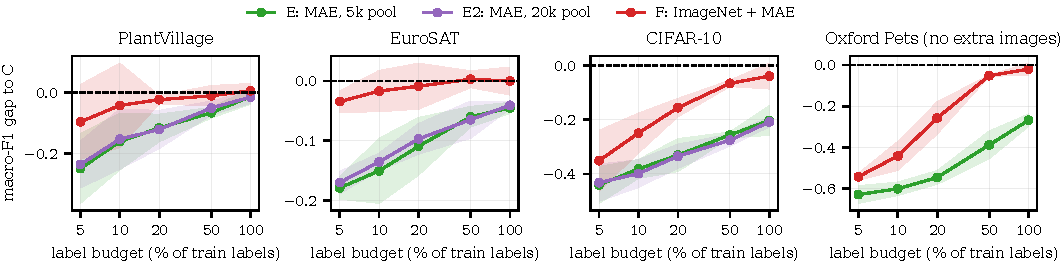
\includegraphics[width=\textwidth]{study2_gaps.pdf}
\caption{Study~2: paired macro-F1 gap to the ImageNet ViT (C) for in-domain MAE on 5,000 images (E), on 20,000
images (E2), and for ImageNet weights with continued MAE (F), with 95\,\% $t$-intervals over three seeds. E2 lies
on top of E. F starts far below C and catches up only when labels are plentiful.}
\label{fig:study2}
\end{figure*}

\begin{table*}[t]
\centering
\caption{Study~2 per dataset, after retuning on the wider learning-rate grid. Mean gaps are averaged over the
log-budget axis (macro-F1). ``sig.\ $+$/$-$'': budgets whose 95\,\% CI lies entirely above / below 0. ``F$>$C /
sig.\ $-$'': budgets where F's mean is higher than C's / budgets where F is significantly lower.}
\label{tab:study2}
\footnotesize
\begin{tabular}{@{}lccccccc@{}}
\toprule
 & E$-$C & \multicolumn{2}{c}{E2$-$E (more unlabelled data)} & E2$-$C & F$-$C & F$>$C / sig.\ $-$ &
A2$-$A (ResNet-34 $-$ 18) \\
\cmidrule(lr){3-4}
Dataset & mean gap & mean gap & sig.\ $+$/$-$ & mean gap & mean gap & (of 5 budgets) & range over budgets \\
\midrule
\tabinput{tables/study2.tex}
\bottomrule
\end{tabular}
\end{table*}

\subsection{A wider learning-rate grid}
With five candidate rates instead of three, the chosen rate changed for 9 of the 16 Study~1 dataset--arm pairs,
and those 135 runs were repeated. The picture did not move. C still won all 20 cells among the original four arms
(H11 supported), and E$-$C stayed negative in all 20, significantly so in 19. The closest call is again
PlantVillage at full labels, now $-0.012$ instead of $-0.020$.

\subsection{Four times more unlabelled images}
If MAE simply had too little data, a bigger pool should have helped. It did not. Across the three datasets that
had extra images, E2 and E differed by at most 0.02 macro-F1 in any cell, E2 was ahead in 8 of 15 cells, and none
of the differences was significant (H6 not supported). E2 also stayed below C in all 15 cells, 14 of them
significantly, and its best result was still 0.014 short (PlantVillage at 100\,\%; H7 not supported). Even the MAE
reconstruction loss barely changed: after the same number of steps it ended at 0.407 rather than 0.409 on
PlantVillage and 0.266 rather than 0.268 on CIFAR-10.

\subsection{ImageNet first, then in-domain MAE}
The hybrid F was meant to take the best of both. It did not. F beat C in only 3 of 20 cells, by at most 0.006 and
never significantly, and it was significantly worse in 10 (H8 not supported). The damage is concentrated at small
budgets. At 5\,\% labels F fell behind C by 0.351 on CIFAR-10 and by 0.542 on Pets, which is most of the advantage
ImageNet had over in-domain MAE. With all labels F recovered to within 0.04 of C everywhere. As expected, F was well
ahead of E2 (by 0.021 to 0.210, significant in 14 of 15 cells; H9 supported), but that edge comes from the ImageNet
start, not from the extra MAE. F also behaved more like a model trained from scratch: it stopped early in 17\,\% of
its runs, close to E (20\,\%) and far from C (67\,\%). Its correlation with the domain distances repeated the pattern
of Study~1, with no $p$ below 0.33.

\subsection{A larger ResNet}
ResNet-34 and ResNet-18 were within 0.03 of each other in 18 of 20 cells. The only significant difference was on
CIFAR-10 with all labels ($+0.042$). Swapping the CNN reversed the comparison with the best MAE arm in a single
cell, so H10 is partly supported, and the claim that MAE roughly matches a scratch CNN at this scale stands.
As for calibration, the mean ECE before temperature scaling was 0.052 for C, 0.116 for E2, 0.146 for F, 0.151 for E
and 0.176 for ResNet-34; after scaling all arms fell between 0.024 and 0.033, as in Study~1.

\begin{table*}[t]
\centering
\caption{All pre-registered hypotheses and their outcomes. H1--H5 were registered before Study~1, H6--H11 before
Study~2.}
\label{tab:hyp}
\footnotesize
\begin{tabular}{@{}lp{7.2cm}p{8.6cm}@{}}
\toprule
 & Hypothesis & Outcome \\
\midrule
H1 & C ahead at small budgets; E closes or reverses the gap at larger budgets &
\textbf{Partly}: the gap closes in all 4 domains, but no crossover up to 100\,\% \\
H2 & Gap E$-$C smaller for domains farther from ImageNet &
\textbf{Not supported}: right direction for 2 of 4 distances, none significant \\
H3 & E $>$ D at every budget in every domain &
\textbf{Mostly}: 20/20 positive, 13/20 significant, none of them on EuroSAT \\
H4 & The best arm differs across domains and budgets ($W < 1$) &
\textbf{Rejected}: C best in 20/20 cells, $W = 0.90$--$1.00$ \\
H5 & Ranking by ECE differs from ranking by macro-F1 &
\textbf{Partly}: similar before temperature scaling, different after \\
\midrule
H6 & A 20,000-image pool improves MAE (E2 $>$ E) on PlantVillage, CIFAR-10 and EuroSAT &
\textbf{Not supported}: differences within $\pm$0.02, 8/15 positive, none significant \\
H7 & E2 narrows the gap to C at every budget and overtakes C somewhere &
\textbf{Not supported}: E2 below C in 15/15 cells (14 significant) \\
H8 & ImageNet + MAE (F) beats C in most cells, more so for distant domains &
\textbf{Not supported}: F $>$ C in 3/20 (none significant), significantly worse in 10/20 \\
H9 & F $\geq$ E2 on the three datasets with a pool &
\textbf{Supported}: F ahead by 0.021--0.210, 14/15 significant \\
H10 & ResNet-34 within 0.03 of ResNet-18 in most cells; MAE-vs-CNN verdict unchanged &
\textbf{Partly}: within 0.03 in 18/20; verdict flips in 1 cell \\
H11 & The wider lr grid does not change the winner among A, C, D, E &
\textbf{Supported}: C still best in 20/20 cells \\
\bottomrule
\end{tabular}
\end{table*}

% =====================================================================================================
\section{Discussion}
\textbf{Why ImageNet keeps winning.} ImageNet-1k holds about 250 times more images than Study~1's in-domain pool and 64
times more than Study~2's, and its labels push the network to pick up shapes, parts and textures. These generic features turn out to be useful
even for leaves and satellite tiles. The ImageNet ViT also learned fastest during fine-tuning and triggered early
stopping in two thirds of its runs. MAE, in contrast, learns by repainting pixels. Its reconstructions
(Fig.~\ref{fig:recon}) get the overall layout right, such as the outline and colour of a leaf, but blur the small
details, including the lesions that separate many PlantVillage classes. That would explain why the gap shrinks as
labels are added: with enough labels, fine-tuning can learn the fine detail that the pretraining objective ignored.

\textbf{Why more unlabelled data did not help.} With 20,000 instead of 5,000 images and the same number of steps,
MAE reached the same reconstruction loss and the same downstream accuracy. At this model size and schedule, the
bottleneck seems to be what pixel reconstruction teaches rather than how many images it sees. Data volumes in the
MAE literature are often orders of magnitude larger~\cite{he2022mae}, so our result says ``four times more does not
help'', not ``more can never help''.

\textbf{Why continued MAE hurt.} Starting MAE from ImageNet weights moved the network away from the
class-level features that made C strong, towards features that are good for repainting pixels. With few labels
there is not enough signal to pull it back, which is why the damage is largest at 5--20\,\% and almost gone at
100\,\%. Two caveats apply. Reed et~al.~\cite{reed2022hpt} saw benefits from such hierarchical pretraining, but they
started from self-supervised weights and used contrastive objectives, not supervised weights and pixel
reconstruction. And our MAE learning rate for F was a fixed guess: F's reconstruction loss stayed above that of the
MAE trained from scratch (0.456 against 0.407 on PlantVillage), so a gentler or shorter schedule might behave
differently. What we can say is that this obvious recipe is not a free improvement.

\textbf{Where in-domain MAE comes closest.} The gap was smallest for the two domains that look least like ImageNet's
object photographs (PlantVillage and EuroSAT) and largest where the content overlaps with ImageNet classes. That
fits the intuition behind H2, yet none of the four distances captured it, so a single number seems too blunt to
forecast a crossover. EuroSAT adds a warning: it had by far the lowest MAE reconstruction loss (0.19, against
0.27--0.54 elsewhere) and the smallest gain over a scratch ViT. A low reconstruction loss is not, by itself, a sign
of a useful representation.

\textbf{What a practitioner can take from this.} With a few thousand to twenty thousand unlabelled images and a
small ViT, start from ImageNet, at every label budget. In domains unlike ImageNet the remaining advantage at full
labels can be small (about one macro-F1 point on PlantVillage), and in-domain MAE is still a clear step up from a
ViT trained from scratch. Calibration should be checked for each domain, because the accuracy ranking does not
carry over to it.

\begin{figure}[t]
\centering
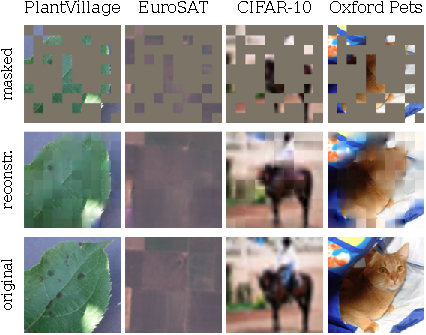
\includegraphics[width=\columnwidth]{mae_reconstructions.pdf}
\caption{MAE reconstructions from Study~1 (seed 0, one training image per domain). Top: input with 75\,\% of the
patches hidden; middle: reconstruction; bottom: original. The layout comes back, fine detail such as leaf lesions
does not.}
\label{fig:recon}
\end{figure}

% =====================================================================================================
\section{Limitations}
The studies were sized for one laptop GPU, and that sets their limits. (i) We used ViT-Tiny at 160\,px and at most
20,000 unlabelled images per domain. Bigger models, higher resolution and much bigger pools favour MAE in the
literature~\cite{he2022mae}, so a crossover may exist beyond our range. (ii) With four domains no rank correlation
can reach $p < 0.083$, so H2 was only explored. (iii) Three seeds leave wide intervals for small effects.
(iv) Even on the wider grid, 16 of the 27 chosen learning rates sit at one of its two ends, so some arms might still
gain from further tuning; since the conclusions hardly moved when the grid was widened, we do not expect this to
reverse them. (v) MAE used one recipe without a search over the masking ratio or the schedule, and F's MAE learning
rate was not tuned. (vi) The DeiT weights were trained at 224\,px and their position embeddings were interpolated to
160\,px; CIFAR-10 and EuroSAT were upsampled from 32 and 64\,px. (vii) Hashing cannot find every near-duplicate, for
example the same leaf photographed from another angle. (viii) ImageNetV2 replaces ImageNet in the distance
measures, Oxford Pets had no extra images for E2, and C benefits from far more pretraining compute than any MAE arm;
we did not equalise compute between arms.

% =====================================================================================================
\section{Conclusion}
We asked when in-domain MAE pretraining overtakes ImageNet initialisation for a small ViT as more labels become
available. Over four domains and two pre-registered studies, the answer is that it does not, anywhere between 5 and
100\,\% of the labels. ImageNet initialisation won all 20 settings. Its lead shrank as labels were added and was
smallest for plant-disease and satellite images, but none of four standard distances predicted where it would be
small. Giving MAE four times more unlabelled data, widening the learning-rate grid and using a deeper ResNet as the
baseline did not change this, and continuing MAE from ImageNet weights made things worse when labels were scarce.
In-domain MAE did reliably improve a ViT trained from scratch and matched a CNN trained from scratch. The natural
next steps are much larger unlabelled pools, larger ViTs and more domains, which would also make it possible to
test the link between domain distance and the crossover budget with real statistical power.

\section*{Reproducibility}
Code, configurations, both pre-registrations, split files, every run's metrics and the experiment logs are
available at\\
{\footnotesize\url{https://github.com/namratapathak0410-pixel/Label-Efficient-Representation-Learning-SSL}}.\\
Models were built with PyTorch and timm~\cite{wightman2019timm}. Every figure and table in this paper is produced
from the result files by \texttt{paper/make\_figures.py}.

% balance the two columns of the last page
\IEEEtriggeratref{23}
\bibliographystyle{IEEEtran}
\bibliography{refs}

\end{document}
